%%% use twocolumn and 10pt options with the amrob format
\documentclass[twocolumn,10pt]{amrob}
\usepackage[utf8]{inputenc}
\usepackage{url}
\usepackage{graphicx}
\usepackage{mathtools}
\usepackage{color}
\usepackage{multirow}

\newcommand{\TODO}[1]{{\color{red}{ToDo: {#1}}}}
\newcommand{\NOTE}[1]{{\color{blue}{Note: {#1}}}}
\newcommand{\EXCISE}[1]{}

\special{papersize=8.5in,11in}

%% The default is oneside, onecolumn, 10pt, final

%%% Replace here with information related to your conference
\confshortname{XVIII COMRob 2016, ISBN: En tr\'amite}
\vspace{0.5mm}
\conffullname{ XVIII Congreso Mexicano de Rob\'otica 2016\\
              Universidad Aut\'onoma de Sinaloa y Asociaci\'on Mexicana de Rob\'otica e Industria AC}

%%%%% for date in a single month, use
%\confdate{1-4}
%\confmonth{Octubre}
%%%%% for date across two months, use
\confdate{9--11 de Noviembre}
\confyear{2016}
\confcity{Mazatl\'an, Sinaloa}
\confcountry{M\'exico}

%%% Replace DETC2009/MESA-12345 with the number supplied to you 
%%% by ASME for your paper.
\papernum{XVIIICOMRob2016/ID-000}

%%% You need to remove 'DRAFT: ' in the title for the final submitted version.

\title{Sistema de Robots Móviles Omnidireccionales para Aplicaciones Colaborativas\thanks{Se agradece el patrocinio a esta investigación de la Asociación Mexicana de Cultura A.C.}}


%%% first author
%\author{Edgar Granados Osegueda 
%    \affiliation{
%	Departamento de Sistemas Digitales \\
%    ITAM\\
%	Rio Hondo 1, Ciudad de México, 01080\\
%    edgar.granados@itam.mx
%    }	
%}

%%% all authors
%%% remove the following entry for single author papers
%%% add more entries for additional authors
\author{Edgar Granados Osegueda \qquad Marco Morales \qquad José Guadalupe Romero
    \affiliation{
    Departamento de Sistemas Digitales, ITAM\\
	Rio Hondo 1, Ciudad de México, 01080\\
	\{edgar.granados,marco.morales,jose.romerovelazquez\}@itam.mx
    }
}

%\author{José Guadalupe Romero
%    \affiliation{
%    Departamento de Sistemas Digitales \\
%    ITAM\\
%	Rio Hondo 1, Ciudad de México, 01080\\
%	jose.romerovelazquez@itam.mx
%    }
%}

\begin{document}
\graphicspath{ {./Figures/} }
\epstopdfsetup{outdir=./Figures/}
\maketitle    

%%%%%%%%%%%%%%%%%%%%%%%%%%%%%%%%%%%%%%%%%%%%%%%%%%%%%%%%%%%%%%%%%%%%%%
\begin{abstract}
{\it 
En este artículo se presenta el diseño y construcción de un sistema de robots móviles omnidireccionales para aplicaciones colaborativas. Además de los mecanismos de movimiento, los robots cuentan con un par FPGA/microcontrolador donde se ejecutan dos lazos de control de velocidad (a nivel de motores y a nivel de robot). Un sistema computacional externo que utiliza la infraestructura del Robot Operating System (ROS) permite la modularización del sistema con facilidades de mantenimiento y extensiones futuras. Este sistema se diseñó con base a las especificaciones de la Small Size League de RoboCup, sin embargo se proyecta usar en otras aplicaciones tanto para investigación como para enseñanza. Los experimentos realizados ilustran el buen comportamiento del sistema diseñado.
}



\end{abstract}
% \\
% \\



%%%%%%%%%%%%%%%%%%%%%%%%%%%%%%%%%%%%%%%%%%%%%%%%%%%%%%%%%%%%%%%%%%%%%%
\section*{INTRODUCCIÓN}

% Problema de investigación/desarrollo
En este trabajo presentamos un sistema de robots para aplicaciones colaborativas. Nuestra aplicación inmediata es la \textit{Robocup Small Size League} pero se puede adaptar fácilmente a otras aplicaciones por su diseño modular. Nuestro sistema está construido sobre el Robot Operating System (ROS) lo cual facilita su mantenimiento y la incorporación de módulos de terceros. 

% Motivación
Las aplicaciones para robots móviles son extensas incluyendo exploración, transporte en ciudades, limpieza y organización de inventarios. Existen diversos tipos de robots móviles incluyendo los humanoides (e.g, el Nao), los voladores y los que se mueven con ruedas. Estos últimos tienen una estructura mecánica y modelos relativamente sencillos \cite{corke2011robotics} por lo que son una  buena opción para realizar tareas sobre superficies  planas. Un caso específico de este tipo de robots es el robot omnidireccional que puede alcanzar cualquier pose en el plano sin restricciones en su trayectoria. Esto lo hace muy útil en ambientes dinámicos con poco espacio para maniobrar o que requieren cambios abruptos de dirección como fábricas, hospitales y almacenes. Por otra parte, en diversas tareas se requiere el trabajo colaborativo de múltiples robots. Este es el caso de la distribución de objetos en inventarios o la supervisión o vigilancia en espacios grandes y complejos. 

% Solución presentada
En este trabajo se presenta una arquitectura modular. Presentamos el sistema mecánico del robot que incluye diseños propios de chasis, ruedas, motores y reductores de velocidad. El sistema electrónico incluye un FPGA, un microcontrolador, un sistema de comunicaciones y circuitos de potencia. El sistema computacional es distribuido entre el robot y un sistema externo modular. El sistema externo usa la infraestructura del Robot Operating System (ROS) y consta de módulos de Visión, Planeación y Control de Regulación. El sistema en el robot determina la acción de control para cada motor. Nuestros experimentos muestran un buen desempeño de todos los sistemas a nivel de motor, a nivel de robot y a nivel de trayectoria tanto en lazo abierto como en lazo cerrado.

\section*{MARCO DE REFERENCIA}
\label{sec:marco_ref}
La principal ventaja de los robots omnidireccionales es su maniobrabilidad. 
Algunos ejemplos interesantes son el OmniBot de la NASA~\cite{houshangi1999omnibot} (altamente maniobrable en ambientes peligrosos), el Airtrax ATX-3000~\cite{aduascualictei2011practical} (levantacargas para almacenes) y la OMNI-chair~\cite{borgolte1998architectural} (silla de ruedas omnidireccional).
Un robot omnidireccional se puede trasladar sobre un plano entre dos poses arbitrarias en trayectorias arbitrarias que le permiten cambios simultaneos de posición y orientación \cite{rojas2005short}. Las poses se caracterizan por una posición $(x,y)$ y una orientación $\theta$ respecto a un sistema de referencia. El movimiento omnidireccional se logra con al menos 3 ruedas omnidireccionales concéntricas colocadas con distintos ángulos de separación \cite{rojas2006holonomic}. Ruedas adicionales proporcionan redundancia  permitiendo mayor tolerancia a fallas, por esto, se suele utilizar cuatro o más ruedas. 

Muchos de los diseños de ruedas omnidireccionales comerciales maximizan la eficiencia de la rueda buscando que el perfil de la rueda sea \textit{perfectamente} circular \cite{rojas2005short}, sacrificando el espacio utilizado por la rueda. La mayoría de los diseños de rueda omnidireccional~\cite{ashmore2002omni} buscan maximizar la eficiencia de la misma aun a costa del espacio utilizado. Por ejemplo, el equipo de RoboCup SSL de Cornell University usó inicialmente ruedas ortogonales~\cite{d2000cornell} compuestas de dos esferas cortadas por dos planos paralelos; el eje de la rueda es perpendicular a las superficies recortadas. Al no proporcionar la tracción necesaria para un control adecuado a altas velocidades las reemplazaron por ruedas omnidireccionales segmentadas~\cite{purwin2003cornell}. Por otro lado, la rueda Mecanum \cite{diegel2002improved} tiene los rodillos en un ángulo en la periferia, pero su diseño es complejo y sus rodillos son muy voluminosos. En contraste, la rueda segmentada tiene los rodillos alineados al eje principal de la rueda permitiendo un diseño compacto.

Los robots en sistemas de este tipo tienen restricciones de tamaño y de consumo de energía. Por esto se han explorado varias opciones para el cómputo a bordo del robot. En algunos casos se usa exclusivamente un FPGA~\cite{chaisoskuba}. En otros casos, se usa uno o más microcontroladores~\cite{rylltigers,egorova2003fu}. También es común usar una combinación de un FPGA y un microcontrolador~\cite{parsian-tdp-2011}.

Este tipo de sistemas incluye mecanismos para operarlos en forma externa desde computadoras remotas. Una opción es utilizar una arquitectura monolítica \cite{mosleh}, pero este tipo de arquitectura  es difícil de mantener. Por el contrario una arquitectura modular facilita el mantenimiento y la expansión de capacidades de un sistema. El \textit{Robot Operating System (ROS)} \cite{quigley2009ros} es un \textit{framework} que permite implementar este tipo de sistemas proporcionando mecanismos para comunicación entre procesos, adem\'as de   librerías especializadas en robótica.
 
\EXCISE{
  El robot presentado en este trabajo se probó inicialmente en el contexto de Robocup \emph{Small Size League} (SSL) \cite{sslWiki}. Los robots deben caber en un cilindro de 18 cm de altura por 15 cm de diámetro y deben moverse sin dañar la carpeta que forma la cancha. La pose de los robots se obtiene con un sistema de visión integrado por cámaras en la parte superior de la cancha además del software provisto por la liga para el procesamiento de imágenes. Esto requiere que los robots tengan un \textit{Patrón Estandar} de colores en su parte superior. En esta competencia, la mayoría de los equipos utiliza un control de velocidad, sin embargo, en 2011, SKUBA presentó un control basado en el torque del motor \cite{chaisoskuba}. 
}

%%%%%%%%%%%%%%%%%%%%%%%%%%%%%%%%%%%%%%%%%%%%%%%%%%%%%%%%%%%%%%%%%%%%
% \section*{DISEÑO DEL ROBOT}
\section*{ARQUITECTURA DEL SISTEMA}
\label{sec:arquitectura_sistema}
% \section*{CONTROLADOR}

El sistema presentado (Fig. \ref{fig:ROSGral}), se diseñó de acuerdo a las reglas y condiciones de juego de la RoboCup SSL, sin embargo esto no limita a los robots para utilizarse en otras aplicaciones. En este sistema, uno o más robots operan en una superficie plana. El módulo de \emph{Visión} determina la pose de cada robot mediante el procesamiento de imágenes entregadas por las cámaras que los monitorean. El módulo de \emph{Planeación} determina la ruta del robot en base a su pose y a la pose deseada. El módulo de \emph{Control} genera trayectoria que debe seguir cada robot y determina su perfil de velocidades para comunicarlo a los robots mediante un enlace inalámbrico. Estos módulos se comunican entre sí mediante ROS. 

%%%%%%%%%%%%%%%% begin figure %%%%%%%%%%%%%%%%%%%
\begin{figure}
  \centering
    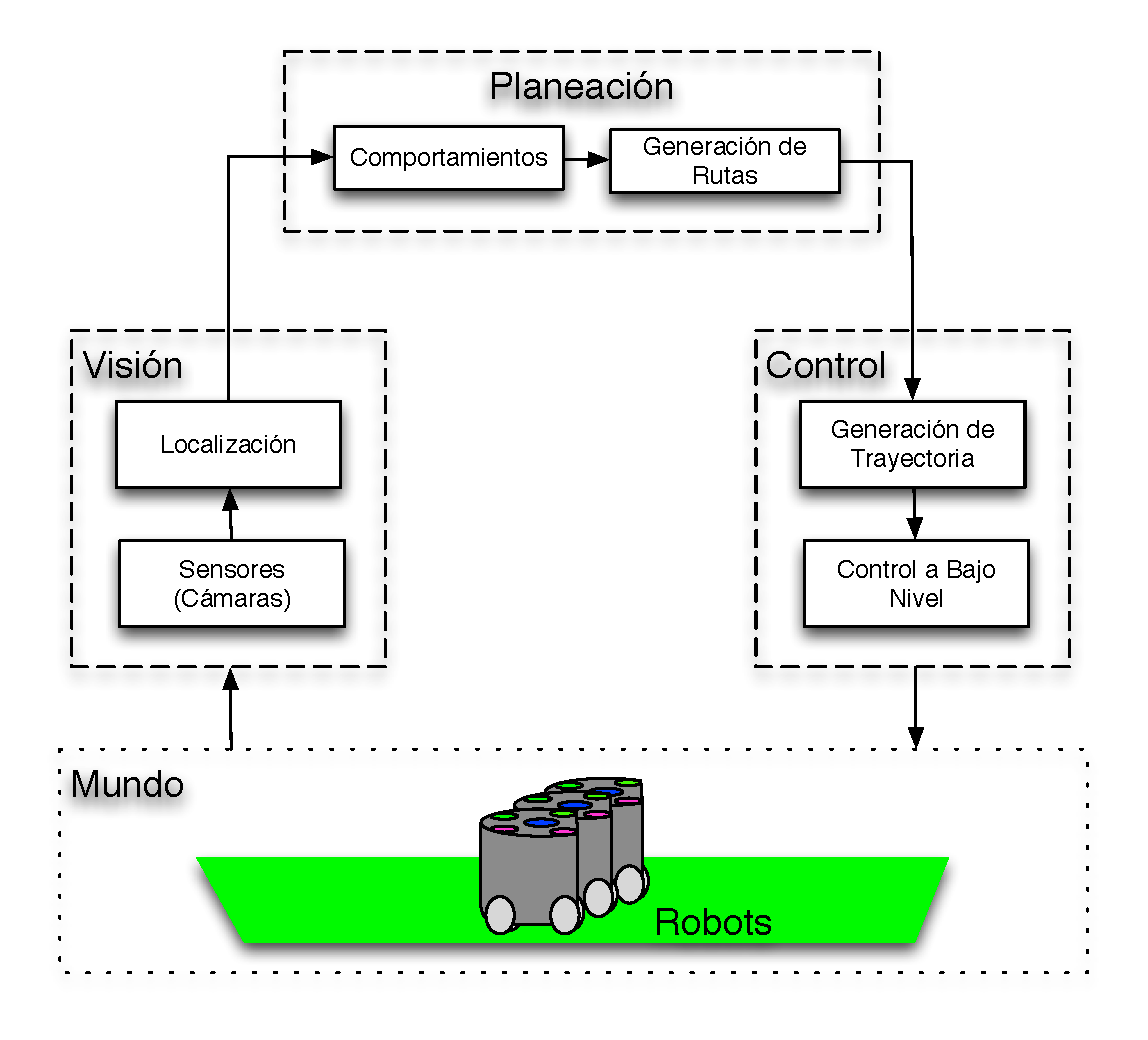
\includegraphics[height=5cm]{arqGeneral.eps}
  \caption{Arquitectura del Sistema}
  \label{fig:ROSGral}
\end{figure}

%%%%%%%%%%%%%%%% end figure %%%%%%%%%%%%%%%%%%% 
\subsection*{Robot}
A continuación describimos el sistema mecánico y el sistema electrónico de cada robot. 
\subsubsection*{Sistema Mecánico}
\label{sec:sistema_movimiento}

Las especificaciones del sistema mecánico son: estructura cilíndrica de un máximo de 18cm de altura por 15cm de diámetro, ruedas concéntricas, peso máximo de 2.5 Kg, velocidad máxima de 3.5 m/s, resistente a colisiones y piezas fácilmente reemplazables.

La estructura se construyó con modelado por deposición fundida (MDF) con dos tipos de plástico: ABS y HIPS. 

El chasis tiene 3 componentes de mayores dimensiones que se manufacturaron con plástico HIPS: base, carcasa y tapa. En la base se ensamblan el resto de los componentes. La carcasa lo protege de impactos. La tapa da soporte al patrón de colores que reconoce el sistema de visión.

Debido a las restricciones en las dimensiones del robot, se realizó un diseño de rueda propio, delgado y con rodillos perpendiculares al eje principal, fácil de ensamblar y resistente. La rueda tiene cuatro piezas únicas, dos de las cuales son de diseño propio: una pieza de plástico ABS (Fig.~\ref{fig:ruedaOmni}) y 21 rodillos de aluminio. Además tiene dos piezas comerciales: 1 cable de acero y 21 orings. Así, el esqueleto es formado por una pieza, lo cual simplifica el ensamblado y la hace más resistente que diseños que utilizan varias piezas como esqueleto. El radio de la rueda (31.5mm) así como el número de rodillos utilizados favorece un funcionamiento eficiente de la rueda comparado con versiones de menor tamaño o menor número de rodillos.

%%%%%%%%%%%%%%%% begin figure %%%%%%%%%%%%%%%%%%%
\begin{figure}[t]
  \centering
    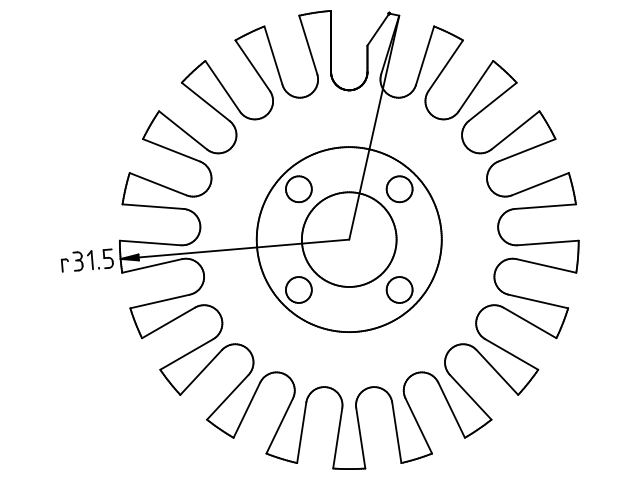
\includegraphics[scale=0.1]{rueda.png}
  \caption{Perfil de Rueda Omnidireccional}
  \label{fig:ruedaOmni}
\end{figure}
%%%%%%%%%%%%%%%% end figure %%%%%%%%%%%%%%%%%%% 

Para cumplir con los requerimientos de velocidad y peso, se utilizan motores sin escobillas y reductores de velocidad. El motor Maxon 200142 tiene una velocidad sin carga de 4370 RPM (nominal de 2940 RPM). El reductor de velocidad está formado por engranes cilíndricos rectos de metal con una razón de reducción de 3.5. Se utilizan engranes comerciales para asegurarse de una construcción con alta eficiencia y ser resistencia a altas velocidades.

La Figura~\ref{fig:ModRealVsdes} muestra el robot real y el modelo en CAD diseñado.
%%%%%%%%%%%%%%%% begin figure %%%%%%%%%%%%%%%%%%%
\begin{figure}
  \centering
    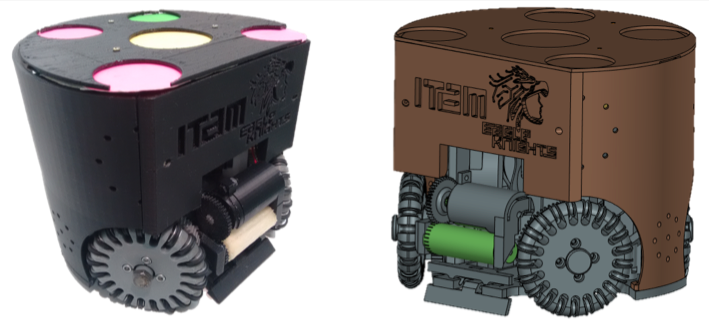
\includegraphics[height=3cm,width=8cm]{realVS3D.png}
  \caption{Robot Real vs Modelo 3D del Robot}
  \label{fig:ModRealVsdes}
\end{figure}
%%%%%%%%%%%%%%%% end figure %%%%%%%%%%%%%%%%%%% 




%%%%%%%%%%%%%%%%%%%%%%%%%%%%%%%%%%%%%%%%%%%%%%%%%%%%%%%%%%%%%%%%%%%%%%
\subsubsection*{Sistema Electrónico}

El sistema electrónico se compone de una tarjeta de desarrollo MOJO, un sistema de comunicaciones y circuitos de potencia para los motores  y de energía para todos los componentes (Fig.~\ref{fig:electGral}). La tarjeta MOJO tiene un FPGA Spartan 6 XC6SLX9 y un microcontrolador ATmega32U4. Las comunicaciones se realizan con XBee WiFi con direccionamiento estático y UDP. Los motores se controlan desde salidas PWM del FPGA mediante un ESC (Electronic Speed Controller) que genera la señal trifásica que requieren. Se utiliza un modelo de ESC dedicado a drones multi-hélice debido a su rapidez de respuesta. Se utilizan dos baterías, una para los motores y ESC's y otra para el resto de la electrónica.

%%%%%%%%%%%%%%%% begin figure %%%%%%%%%%%%%%%%%%%
\begin{figure}
  \centering
    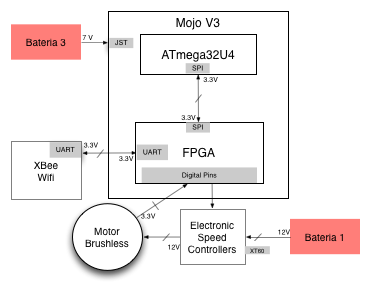
\includegraphics[height=3cm]{diagrama_electronica.png}
  \caption{Componentes electrónicos}
  \label{fig:electGral}
\end{figure}
%%%%%%%%%%%%%%%% end figure %%%%%%%%%%%%%%%%%%%


%%%%%%%%%%%%%%%%%%%%%%%%%%%%%%%%%%%%%%%%%%%%%%%%%%%%%%%%%%%%%%%%%%%%%%
\subsection*{Cómputo}
\label{sec:sistema_computo}
El cómputo se encuentra distribuido entre el robot y un sistema externo. El sistema externo, implementado en ROS, determina la velocidad deseada del robot y consta de los módulos de Visión, Planeación y Control de Regulación (parte del control). El sistema del robot, implementado en el microcontrolador y el FPGA, recibe la velocidad deseada y determina la acción de Control para cada motor.

\subsubsection*{Visión}
\label{subsec:vision}
Se realizó una interfaz con ROS para el sistema de visión de la RoboCup SSL. Procesa la imagen de las cámaras colocadas en la parte superior del espacio de trabajo para determinar la pose de cada robot a 25 Hz.

%%%%%%%%%%%%%%%%%%%%%%%%%%%%%%%%%%%%%%%%%%%%%%%%%%%%%%%%%%%%%%%%%%%%%%
\subsubsection*{Planeación}
\label{subsec:Planificacion}
Este componente es el encargado de realizar la planificación de tareas y de movimientos para todos los robots. La planificación de tareas se encarga de asignar poses meta a cada robot en base a un rol que tengan asignado. La planificación de movimientos identifica rutas libres de colisión para que cada robot llegue a la pose asignada por el planificador de tareas y genera una secuencia de poses que debe visitar en orden. Para evitar obstáculos, a partir de puntos aleatorios fuera de obstáculos, se traza el camino más corto de la posición actual del robot a la meta deseada. 

%%%%%%%%%%%%%%%%%%%%%%%%%%%%%%%%%%%%%%%%%%%%%%%%%%%%%%%%%%%%%%%%%%%%%%
\subsubsection*{Control}
\label{subsec:Ctrl}
El control está dividido en un módulo en ROS para control de regulación y en un controlador a nivel de robot.

%%%%%%%%%%%%%%%%%%%%%%%%%%%%%%%%%%%%%%%%%%%%%%%%%%%%%%%%%%%%%%%%%%%%%%
\subsubsection*{Generación de Trayectorias (Control de Regulación)}
En cada iteración, se genera un perfil de velocidades para enviar el control a nivel de robot. Dada la pose deseada definida por el planeador, el tiempo disponible para lograrla y la pose actual del robot, se traza una recta entre ambas y se discretiza en segmentos de un tamaño similar al del robot. De ahí se define una velocidad para llegar al siguiente segmento.
 Las trayectorias se generan para mover al robot de su pose actual a la deseada. La trayectoria resultante se discretiza y se envía al robot en forma de un perfil de velocidades ($v_x,v_y,v_\theta$).
%%%%%%%%%%%%%%%%%%%%%%%%%%%%%%%%%%%%%%%%%%%%%%%%%%%%%%%%%%%%%%%%%%%%%%
\subsubsection*{Control a Nivel de Robot}
\label{sec:comunicaciones}
El robot recibe el vector de velocidades $V_l= \begin{pmatrix} v_x & v_y & \omega \end{pmatrix}^{T}$ cuyos componentes son guardados en registros del FPGA. También en el FPGA, se implementó un velocímetro digital cuyas entradas son las señales de los sensores Hall de cada motor para calcular el vector de velocidades de motores 
$V_r= \begin {pmatrix} vr_1 & vr_2 & vr_3 & vr_4 \end{pmatrix}^{T} $
cuyos componentes también son guardados en registros. El FPGA envía las velocidades deseadas y las reales al microcontrolador mediante SPI y Memory Mapping. 


Antes de describir el esquema de control utilizado, presentamos las ecuaciones para obtener aceleración traslacional y rotacional y para mapear el vector de velocidades de robot a velocidades de motor,  generadas a partir de \cite{rojas2006holonomic}.

Utilizando la ecuación general de fuerza \( F = Ma \), para cuatro motores, se obtiene la aceleración traslacional $ a = \frac{1}{M}\left(F_1+F_2+F_3+F_4\right)$. Como se muestra en la Fig. \ref{fig:angFzaDiag} cada motor aporta fuerza en $X$ y en $Y$. La aportación del motor 1 la describe $Ma_{1x} = \mid f_1 \mid \cos\left(90 - \varphi_1\right) =  \mid f_1 \mid  \sin\left(\varphi_1\right)$ y $Ma_{1y} = \mid f_1 \mid \cos\left(\varphi_1\right)$. La aportación de los demás motores se obtiene de manera similar.

%%%%%%%%%%%%%%%% begin figure %%%%%%%%%%%%%%%%%%%
\begin{figure}
  \centering
    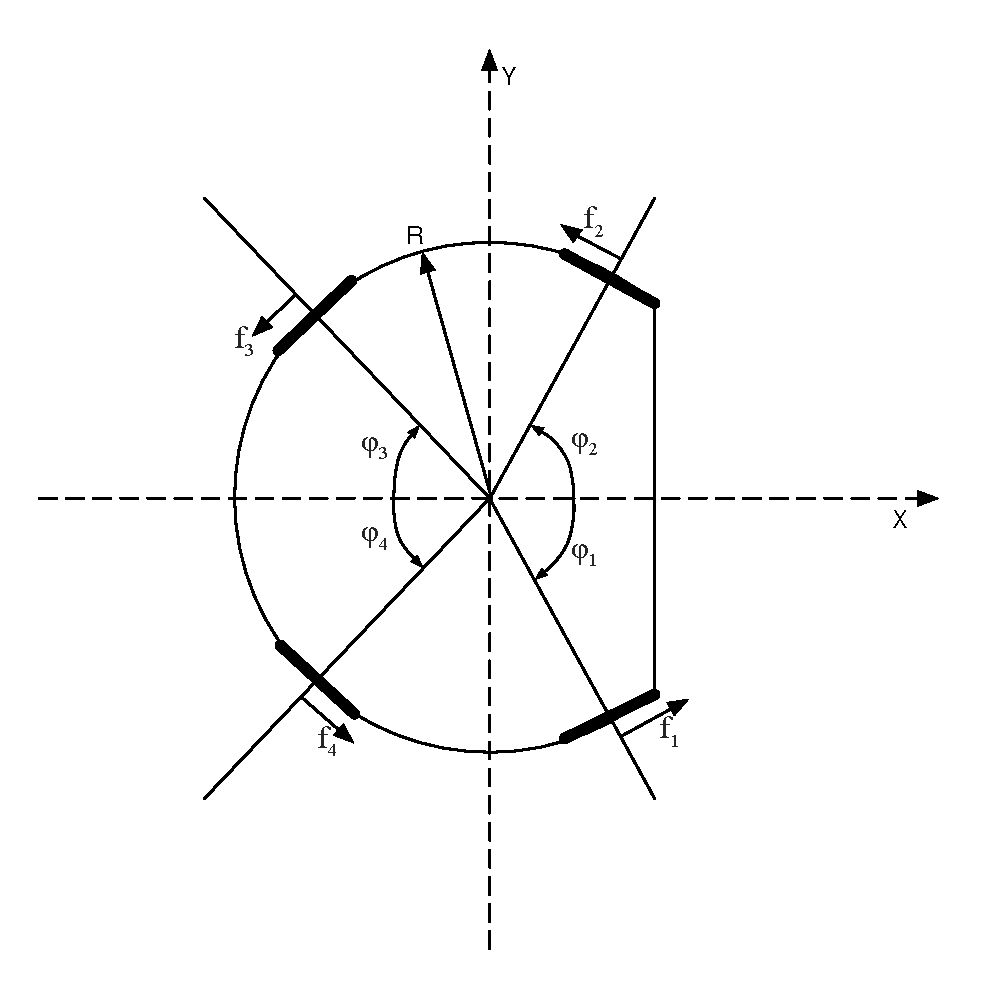
\includegraphics[height=6cm]{anglesRobot.eps}
  \caption{Distribución de Ángulos y Fuerzas}
  \label{fig:angFzaDiag}
\end{figure}
%%%%%%%%%%%%%%%% end figure %%%%%%%%%%%%%%%%%%%

Para obtener la aceleración angular para cuatro motores, de \(\dot{\omega} = \frac{Rf}{I}\) se obtiene  $\dot{w} =\frac{R}{I}\left(f_1+f_2+f_3+f_4\right)$. Sustituyendo el momento de inercia $I = \alpha M R^{2} \mid 0\leq \alpha \leq1$ para un cilindro con distribución de masa desconocida en $\dot{w}$  se obtiene  $R\dot{\omega} = \frac{1}{M\alpha}\left(f_1+f_2+f_3+f_4\right)$.

De estos resultados obtenemos la Eqn.~(\ref{eq:matAcoFzas}) que  tambien se puede expresar como $a=C_\alpha F$, donde $C_\alpha$ es la Matriz de acoplamiento de fuerzas.
%%%%%%%%%%%%%%%% begin equation %%%%%%%%%%%%%%%%%%%
\begin{equation}
  \left(\begin{array}{c}
    a_x \\ a_y \\R_{\dot{\omega}}
  \end{array}\right)= \frac{1}{M}
  \begin{bmatrix}
    \sin\varphi_1 & -\sin\varphi_2 & -\sin\varphi_3 & \sin\varphi_4 \\
    \cos\varphi_1 & \cos\varphi_2 & -\cos\varphi_3 & -\cos\varphi_4 & \\
    \frac{1}{\alpha} & \frac{1}{\alpha}  & \frac{1}{\alpha}  &\frac{1}{\alpha} 
  \end{bmatrix}
  \left(\begin{array}{c}
    f_1 \\ f_2 \\ f_3 \\ f_4  \label{eq:matAcoFzas}\\ 
  \end{array}\right) 
\end{equation}
%%%%%%%%%%%%%%%% end equation %%%%%%%%%%%%%%%%%%%
Para mapear la velocidad deseada $V_{l}'$ al espacio de velocidad de motores deseada $V_m= \begin {pmatrix} v_1 & v_2 & v_3 & v_4 \end{pmatrix}^{T} $. Se considera el perímetro de la rueda y el factor de reducción mediante $V_{l}^{'} = \frac{ V_l \cdot e } { 2 \pi r}$. Así, se obtienen las ecuaciones de cada motor mediante la Eqn. \eqref{eq:velsMots}  y su forma reducida $v_m = D V_{l}^{'}$ donde $D$ es la Matriz de acoplamiento de velocidades. 
%%%%%%%%%%%%%%%% begin equation %%%%%%%%%%%%%%%%%%%
\begin{equation}
  % v_1 = v_x \sin\varphi_1 + v_y\cos\varphi_1 + R \omega \label{eq:velMot1}\\
  v_m = 
    \left(\begin{array}{c}
      v_1 \\ v_2 \\ v_3 \\ v_4 
    \end{array}\right)
    = 
    \begin{bmatrix}
      \sin\varphi_1 & \cos\varphi_1 & 1 \\
      -\sin\varphi_2 & \cos\varphi_2 & 1 \\
      -\sin\varphi_3 & -\cos\varphi_3 & 1 \\
      \sin\varphi_4 & -\cos\varphi_4 & 1 \\
    \end{bmatrix}
    \left(\begin{array}{c}
      v_x^{'}  \\ v_y^{'}  \\ {Rw}^{'} 
    \end{array} \right) \label{eq:velsMots} \\
\end{equation}
%%%%%%%%%%%%%%%% end equation %%%%%%%%%%%%%%%%%%%

En la Figura \ref{fig:ctrl} se muestra el esquema de control implementado. Primero, un control PI determina un vector $V_l'$ que se mapea a las velocidades de motor deseadas $V_m$. 
A continuación, se aplica un segundo control PI a cada motor cuya  salida se envía a la FPGA para convertirla a una señal PWM  y alimentarla al ESC correspondiente. La velocidad real de cada motor se lee de la FPGA como retroalimentación del segundo ciclo de control. Adicionalmente, utilizando la matriz de acoplamiento inversa se obtiene el vector de velocidades reales $(X'$ $, Y'$ $, \theta')$ que utiliza el primer control PI.
%%%%%%%%%%%%%%%% begin figure %%%%%%%%%%%%%%%%%%%
\begin{figure}
  \centering
    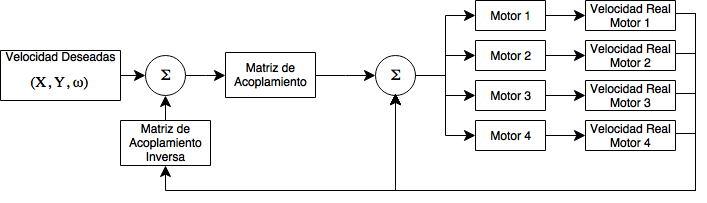
\includegraphics[width=9cm]{ciclo_ctrl_avr.png}
  \caption{Esquema de Control Implementado}
  \label{fig:ctrl}
\end{figure}
%%%%%%%%%%%%%%%% end figure %%%%%%%%%%%%%%%%%%% 

% \subsubsection{Control PI}
%%%%%%%%%%%%%%%%%%%%%%%%%%%%%%%%%%%%%%%%%%%%%%%%%%%%%%%%%%%%%%%%%%%%%%
% \subsection{ROS}
% Aunque el sistema está implementado con ROS, el robot no depende de su utilización. El sistema implementado está enfocado a SSL pero la arquitectura se diseñó para poder intercambiar módulos dependiendo del problema planteado. A continuación describimos los componentes de nuestro sistema de software.
%%%%%%%%%%%%%%%%%%%%%%%%%%%%%%%%%%%%%%%%%%%%%%%%%%%%%%%%%%%%%
% \section*{ALGORITMOS}
% \label{sec:algoritmos}
% En esta sección se describen los algoritmos implementados en el sistema de software para determinar rutas y trayectorias y en el robot, para el control de bajo nivel.

% \subsection*{Control de Bajo Nivel del Robot}
% \subsubsection*{Movimiento Omnidireccional}
% \label{subsec:mov_omni}
%%%%%%%%%%%%%%%%%%%%%%%%%%%%%%%%%%%%%%%%%%%%%%%%%%%%%%%%%%%%%%%%%%%%%%
% \subsubsection*{Control}
% \label{subsec:algoritmos-ctrl}
% El esquema general del algoritmo de control utilizado se muestra en la Fig. \ref{fig:ctrl}. Se implementó un primer control PI a nivel de cada motor. Un segundo ciclo de control se implementó a nivel de robot utilizando la matriz de acoplamiento inversa y las velocidades reales de los motores para obtener el vector de velocidades reales $(X, Y, \theta)$.   La sintonización de las variables se realiza a mano. \par
% % Se incorporó un PI a nivel motor, utilizando el método de Ziegler - Nicholson para realizar la sintonización de las variables.
% Adicionalmente, se cuenta con la retroalimentación de la visión gracias a la cual se puede calcular y corregir la trayectoria del robot al enviar continuamente actualizaciones de la velocidad deseada (30 Hz). 
% % En la Fig. \ref{fig:visionPrueba} se muestran las trayectorias seguidas por el robot al utilizar solamente el control PI así como utilizando el control PI y la retroalimentción de la visión.
%%%%%%%%%%%%%%%%%%%%%%%%%%%%%%%%%%%%%%%%%%%%%%%%%%%%%%%%%%%%%%%%%%%%%%
%%%%%%%%%%%%%%%%%%%%%%%%%%%%%%%%%%%%%%%%%%%%%%%%%%%%%%%
% \subsection*{Algoritmos de Planeación y Control} \NOTE{Buscar un mejor nombre para la sección}
%%%%%%%%%%%%%%%%%%%%%%%%%%%%%%%%%%%%%%%%%%%%%%%%%%%%%%%%%%%%%%%%%%%%%
\section*{EXPERIMENTOS Y RESULTADOS}
\label{sec:experimentacion_resultados}
A continuación se presentan experimentos para evaluar el desempeño de nuestro sistema. Primero hacemos pruebas a nivel de robot para observar  el comportamiento de los lazos internos de control, el que opera a nivel de velocidades de motor y el que opera a nivel de velocidad de robot. Después seguimos con experimentos a nivel de sistema en donde determinamos la capacidad del sistema de alcanzar poses a lazo abierto y después a lazo cerrado y con trayectorias dinámicas.

%%%%%%%%%%%%%%%% end table %%%%%%%%%%%%%%%%%%% 
% Con el diseño propuesto se logra que el robot se mueva aproximadamente a la velocidad propuesta, manteniendo la integridad de sus componentes y con un peso menor que el contemplado inicialmente, aunque siendo capaz de cargar los 3.5 Kg propuestos. Tanto la carcasa como la base y las ruedas han sido capaces de resistir golpes entre los robots a las velocidades normales de movimiento y la visión reconoce el patrón estandar incoporado en la carcasa. En la Fig. \ref{fig:ModRealVSdes} se muestra una comparación entre el diseño modelado en 3D y la construcción final del robot.\par 
\EXCISE{
  En la Fig. \ref{fig:realVSdes} se muestra la respuesta de los motores ante una velocidad deseada con el control PI implementado. 

  Estableciendo 8 direcciones en el plano XY, se obtuvo la respuesta del robot en cada dirección con control PI sin visión y con visión como se puede ver en la Fig. \ref{fig:visionPruebasRetro}. Para el caso de la retroalimentación de visión, existen algunas direcciones en las cuales el movimiento y su posición final es cercano al deseado, especificamente en las direcciones en que prácticamente sólo se utilizan dos ruedas. En cambio en las otras direcciones, se tiene mayor error en el movimiento del robot. Para el caso del movimiento con retroalimentación de visión, aunque en algunos casos existe un movimiento errático, la posición final es muy cercana a la deseada gracias a la correción que realiza el sistema ante los errores en el movimiento del robot.

  Utilizando los datos del experimento anterior, se obtener el error en el tiempo definido como la diferencia entre la posición deseada y la medida, en la Fig. \ref{fig:errorPlot} se puede observar la mejora que representa la retroalimentación de visión. Se puede observar como el error en las trayectorias sin visión es incremental mientras que en las trayectorias con visión, el error alcanza un máximo para disminuir, alcanzando la posición deseada.
}

\subsection*{Pruebas a nivel de robot}
En estas pruebas el robot recibe un vector de velocidad deseada $(X, Y,\theta)$ cuyos parámetros se fijan en uno de los siguientes valores: $+V_{cte}, 0, -V_{cte}$. Existen 27 posibles combinaciones que se aplican en secuencias espaciadas en intervalos de 10s para medir la respuesta de los motores en dos escenarios como se muestra en la Fig.~\ref{fig:realVSdes}. Primero evaluamos el lazo de control a nivel de motor manteniendo abierto el lazo de control a nivel de robot. Solo en algunos casos no se alcanzan las velocidades de robot deseadas. Esto sucede cuando la velocidad de motor requerida es superior a la \emph{no-load speed} del motor ,$(+V, +V, +V )$ y $(-V, -V, -V) $ para el motor 1. También sucede cuando la velocidad de motor requerida es muy baja se presentan oscilaciones alrededor de esta, $(+V, -V, 0) $ y  $(+V, -V, -V)$. Después evaluamos el lazo de control a nivel de robot que determina la velocidad requerida al lazo de control a nivel de motor, por lo que esta última no es constante. En todos los casos se alcanzan y mantienen las velocidades de robot independientemente de que se consigan  las velocidades requeridas de motor. En algunos casos, $(+V, +V, +V )$ y $(+V, +V, -V)$, la respuesta es lenta aunque esto se puede mejorar sintonizando $k_p$ y $k_i$.

% \NOTE{En la imagen \ref{fig:realVSdes} se podría cambiar a que sea solamente una entrada y su respuesta?}
%%%%%%%%%%%%%%%%%%%%%%%%%%%%%%%%%%%%%%%%%%%%%%%%%%%%%%%%%%%%%%%%%%%%%%
%%%%%%%%%%%%%%%% begin figure %%%%%%%%%%%%%%%%%%%
\begin{figure}
  \centering
    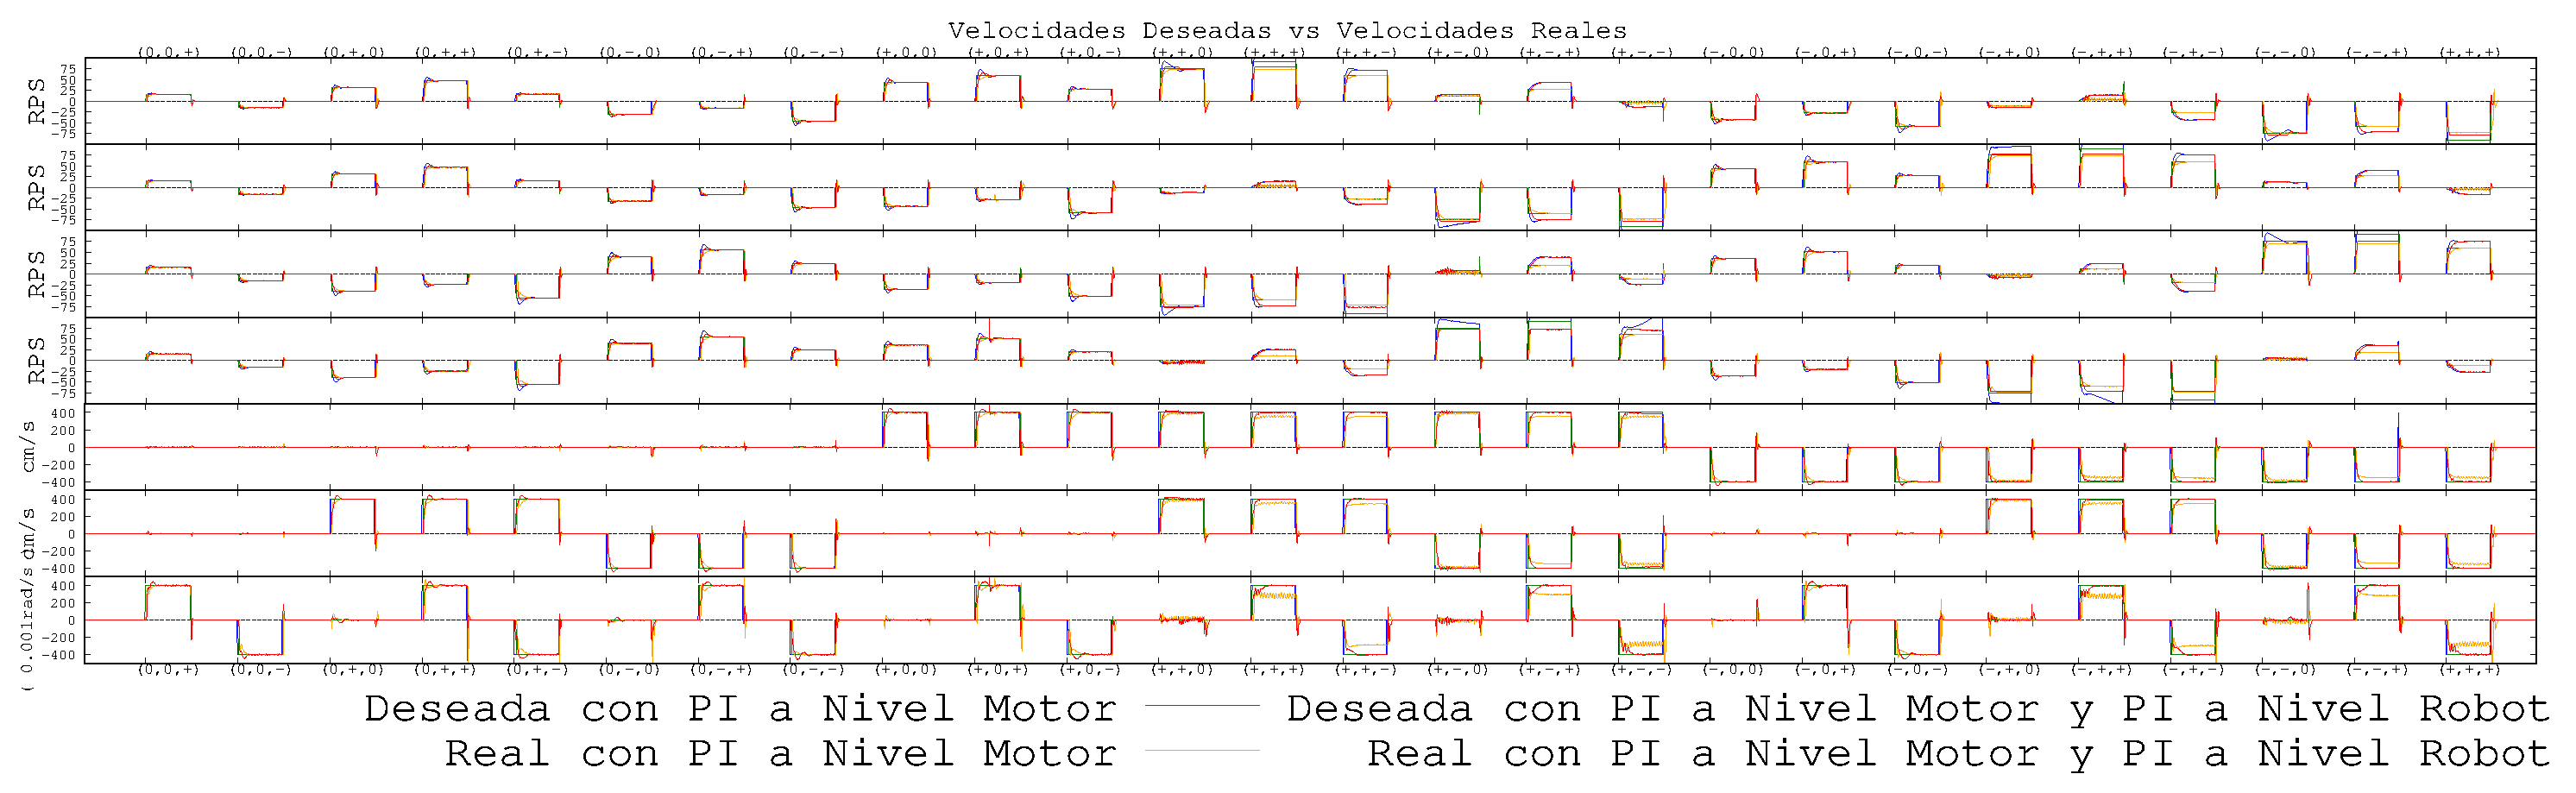
\includegraphics[height=5cm,width=8cm]{160517-vels-motVSmotrob.eps}
  \caption{Velocidades de deseada y real de: motores 1, 2, 3 y 4. A nivel Robot $V_x$, $V_y$ y $V_\theta$. }
  \label{fig:realVSdes}
\end{figure}
%%%%%%%%%%%%%%%% end figure %%%%%%%%%%%%%%%%%%% 
%%%%%%%%%%%%%%%%%%%%%%%%%%%%%%%%%%%%%%%%%%%%%%%%%%%
\subsection*{Pruebas a Nivel Sistema} 
En estas pruebas se establecen puntos que el robot debe alcanzar y se utiliza el sistema computacional externo para definir los perfiles de velocidad. Como se muestra en la Fig. \ref{fig:8pts_without_vision}, se define una circunferencia con centro en $P_0$ y 8 puntos ${P_A, P_B, ..., P_H}$ en la circunferencia tales que: $\angle P_nP_0P_{n+1} = 45^\circ $. La prueba realizada consiste en colocar al robot en $P_0$, siempre orientado a $P_C$. Se calcula la velocidad $(V_x,V_y,\omega)$ para dirigir el robot a cada uno de los 8 puntos. 

%%%%%%%%%%%%%%%% begin figure %%%%%%%%%%%%%%%%%%%
\begin{figure}
  \centering
    \includegraphics[height=8cm,width=8cm]{8pts260517-without-vision.eps}
  \caption{Trayectorias sin retroalimentación}
  \label{fig:8pts_without_vision}
\end{figure}
% \subsubsection*{Pruebas sin Retroalimentación de Visión}
\label{subsec:exper_res-pruebas_sin_vision}
%%%%%%%%%%%%%%%%%%%%%%%%%%%%%%%%%%%%%%%%%%%%%%%%%%%%%

\subsubsection*{Pruebas sin retroalimentación de visión}
En estas pruebas el sistema computacional externo se usa para capturar poses del robot y generar la velocidad inicial deseada. La Fig. \ref{fig:8pts_without_vision} muestra las trayectorias ideales y 10 repeticiones de trayectorias reales. Cada punto representa el centro del robot.

%%%%%%%%%%%%%%%%%%%%%%%%%%%%%%%%%%%%%%%%
%\subsubsection*{Movimiento en el Plano}
%%%%%%%%%%%%%%%%%%%%%%%%%%%%%%%%%%%%%%%%

En movimiento translacional, se obtuvo el mejor desempeño en dirección al punto $P_C$ y a $P_G$ en que mantiene líneas casi rectas. En dirección a $P_B$ y a $P_D$ las trayectorias son curvas, cruzando al vector de dirección ideal. En dirección a $P_F$ y $P_H$ tenemos los mayores errores aunque el ciclo de control a nivel robot corrige el movimiento para llegar al punto objetivo. Las trayectorias hacia  $P_A$ y $P_E$ presentan el peor desempeño sin alcanzar el punto objetivo en ninguna ocasión. 


%%%%%%%%%%%%%%%% end figure %%%%%%%%%%%%%%%%%%%
%%%%%%%%%%%%%%%%%%%%%%%%%%%%%% 
% \subsubsection*{Orientación}
% %%%%%%%%%%%%%%%%%%%%%%%%%%%%%%
% A partir de los mismos datos utilizados en la subsección pasada, en la Fig. \ref{fig:orient_without_vision}
% se muestra el error en la orientación para cada prueba realizada a cada punto. Los datos presentan saltos debido a que solo se presenta la orientación durante el movimiento del robot de $P_0$ al punto deseado, no del reposicionamiento a $P_0$.
% \par

En movimiento rotacional, se mantuvo la velocidad angular en 0 para mantener la orientación del robot. Se obtuvo el mejor desempeño en dirección a los puntos $P_C$ y $P_G$. En dirección a $P_B, P_D, P_F$ y $P_H$, el error es mayor aunque en la mayoría de los casos es menor a 0.5 radianes. Solo en dirección a $P_A$ y $P_E$, el error llega a sobrepasar los 0.5, aunque es mayor en las trayectorias al punto $P_A$. 

% %%%%%%%%%%%%%%%% begin figure %%%%%%%%%%%%%%%%%%%
% \begin{figure}
%   \centering
%     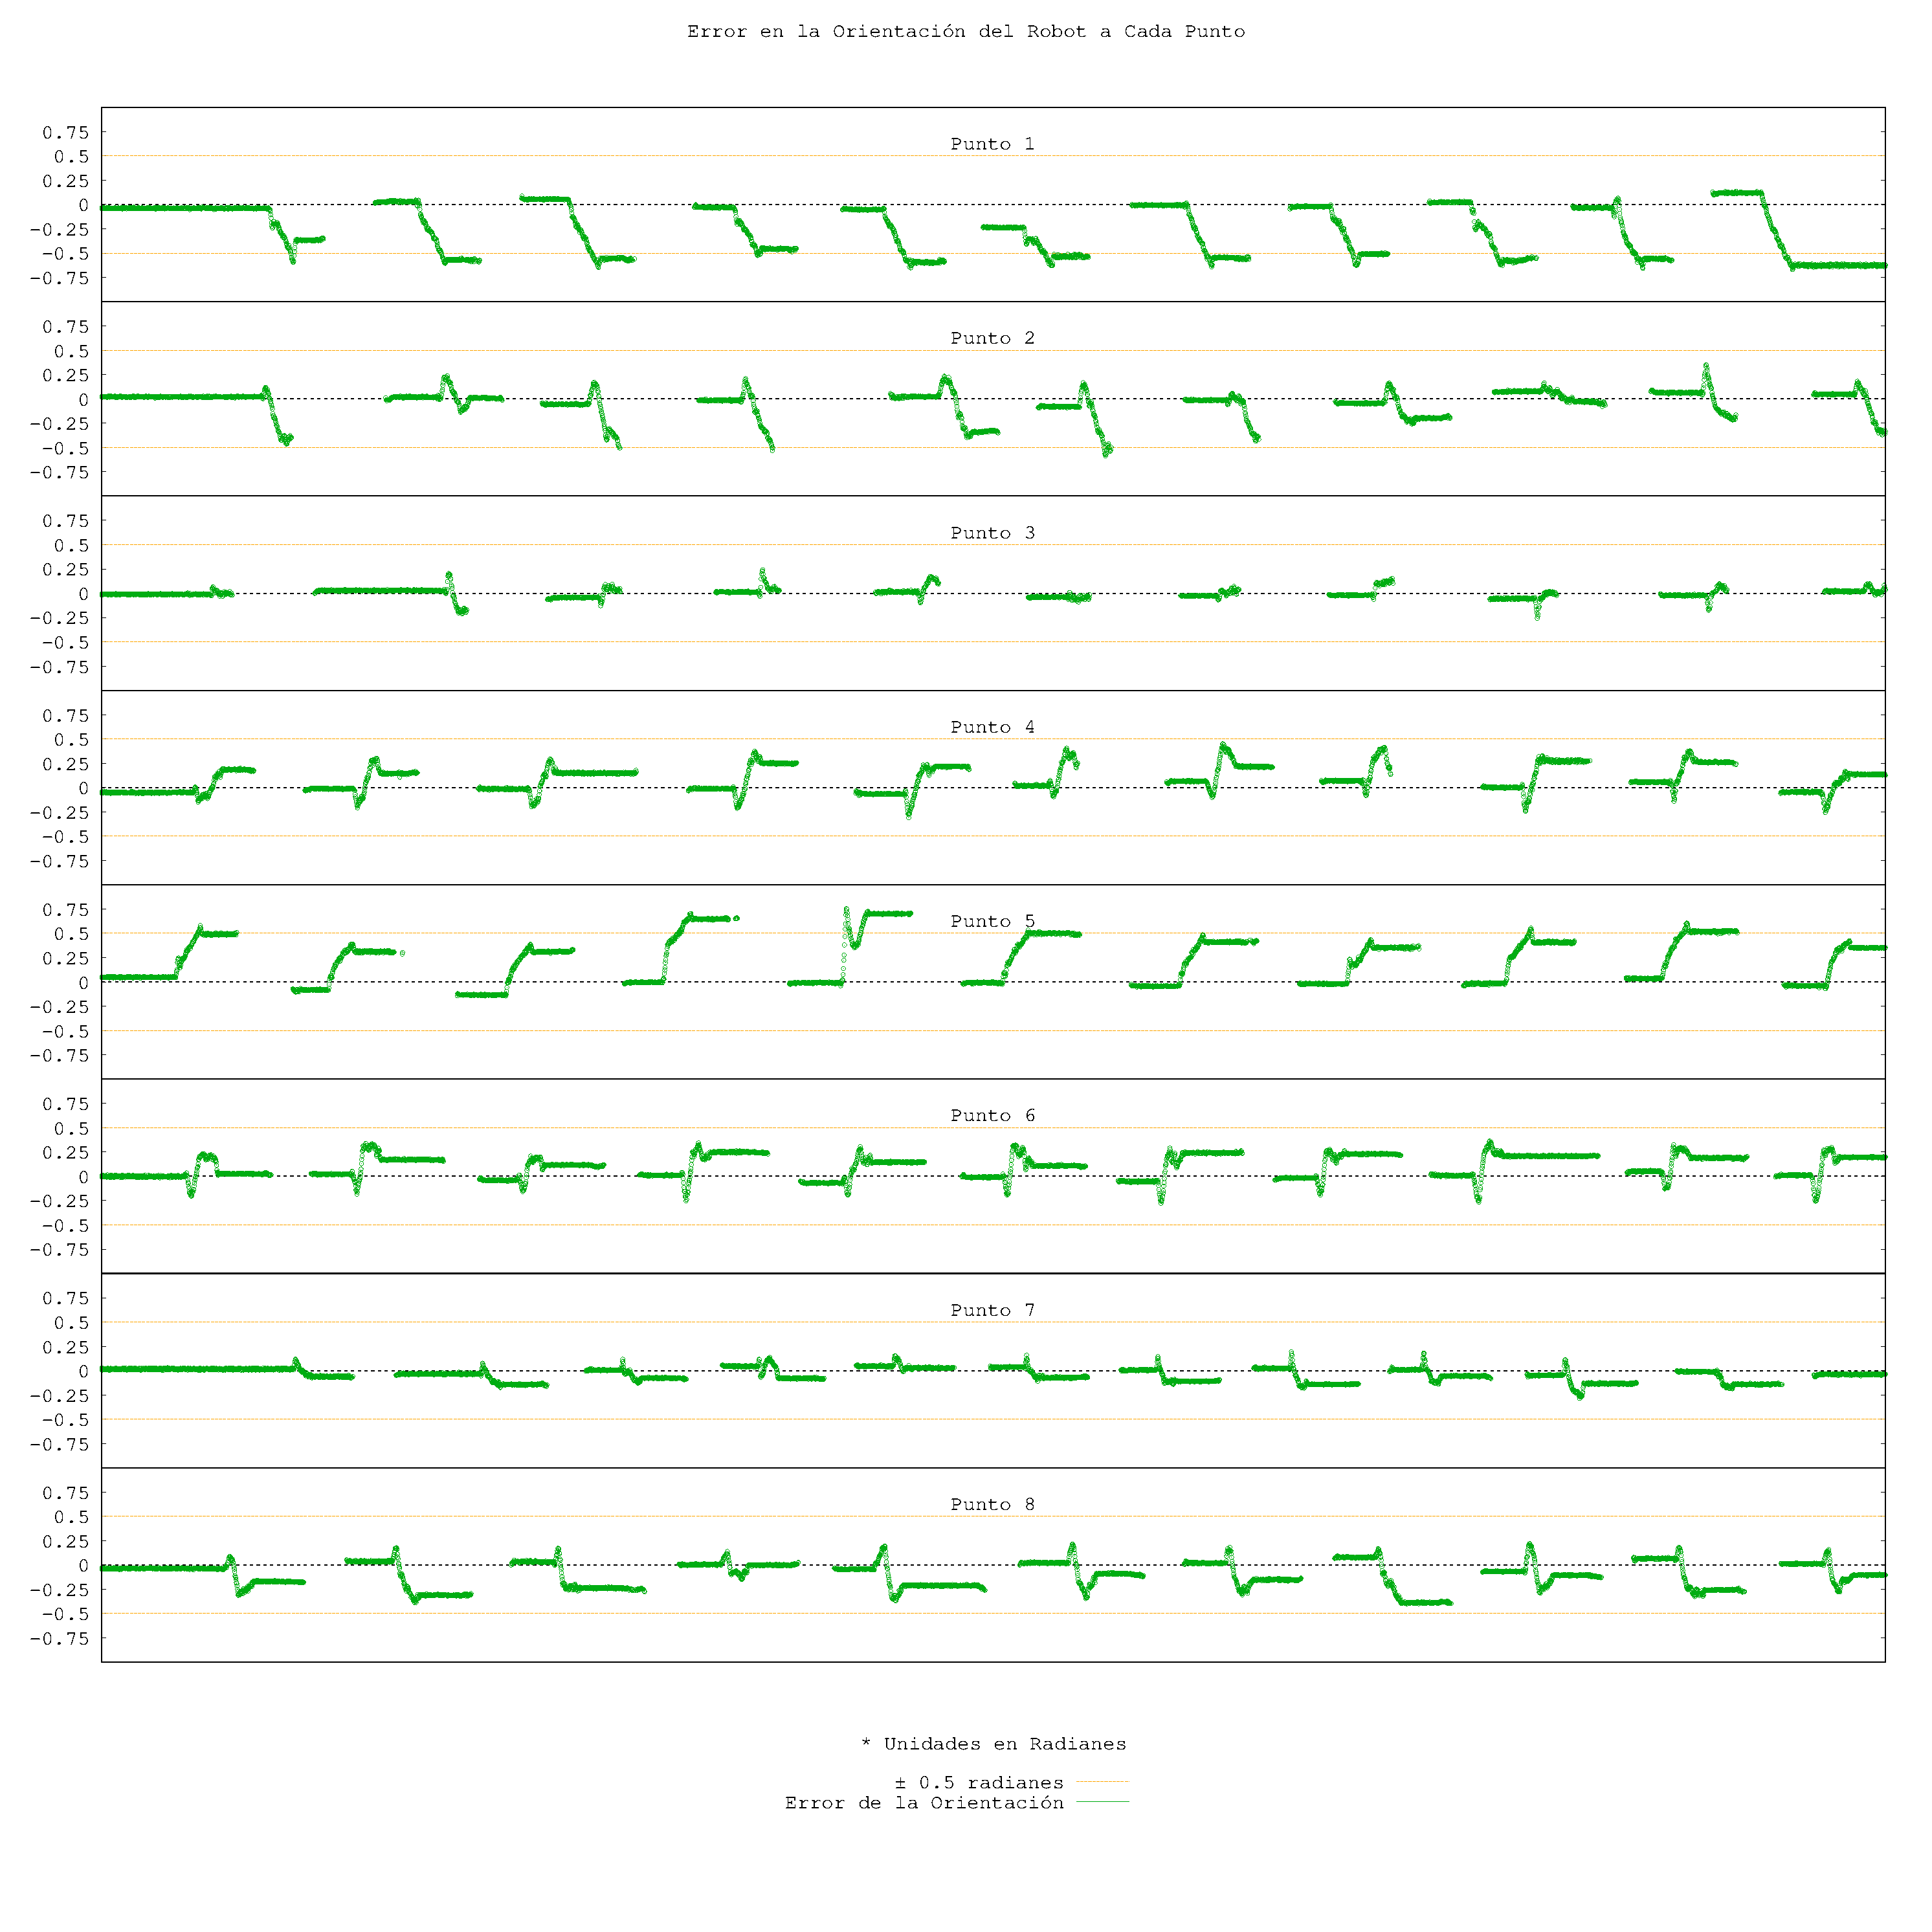
\includegraphics[height=3cm,width=8cm]{8pts260517-without_vision-multi-theta.eps}
%   \caption{Error en la Orientación del Robot en las Pruebas sin Retroalimentación de Visión}
%   \label{fig:orient_without_vision}
% \end{figure}
%%%%%%%%%%%%%%%% end figure %%%%%%%%%%%%%%%%%%% 
%%%%%%%%%%%%%%%%%%%%%%%%%%%%%%%%%%%%%%%%%%%%%%%%%%%%%%%%%%%%%%%%%%%%%%%%%%%%%%%%%%%%%%%%
\subsubsection*{Pruebas con Retroalimentación de Visión y Trayectoria Dinámica}
\label{subsec:exp_res-pruebas_vision}
%%%%%%%%%%%%%%%%%%%%%%%%%%%%%%%%%%%%%%%%%%%%%%%%%%%%%%%%%%%%%%%%%%%%%%%%%%%%%%%%%%%%%%%%
El objetivo de éstas pruebas es validar el movimiento del robot ante un ambiente dinámico donde la trayectoria deseada cambia rápidamente. En estas pruebas el módulo de planeación genera la siguiente pose objetivo y define una ruta viable (una recta al no existir obstáculos). El módulo de control sigue la trayectoria en un esquema de regulación que actualiza los puntos al acercarse a una distancia mínima y genera el vector de velocidad deseada del robot $(X, Y, \theta)$. El robot colocado inicialmente en $P_0$ visita cada punto en la secuencia $(P_A, P_0, P_B, P_0, ..., P_G, P_0, P_H, P_0)$ mientras mantiene la orientación en dirección a $P_C$. 

%%%%%%%%%%%%%%%%%%%%%%%%%%%%%%%%%%%%%%%%
%\subsubsection*{Movimiento en el Plano}
%%%%%%%%%%%%%%%%%%%%%%%%%%%%%%%%%%%%%%%%
% En la Fig. \ref{fig:8pts_vision_multi} se muestra la respuesta del robot en las 10 pruebas realizadas. Para cada prueba, se grafica la trayectoria deseada (generada por el módulo de control) así como la trayectoria real seguida por el robot. 
En movimiento translacional, debido a los cambios en el tiempo de los puntos intermedios, las trayectorias no necesariamente son rectas. Sin embargo, el robot siempre alcanza los puntos deseados. En movimiento rotacional, el error es mínimo solo llegando en una ocasión a ser de 1 radian. La tabla~\ref{tab:SinVisionConVision} muestra una comparación de la norma cuadrada de los errores en pose $(e_X,e_Y,e_\theta)$ que muestra el mejor desempeño esperado cuando se usa retroalimentación con visión. En la mayoría de los casos el error a lazo abierto es de 3 a 5 veces el obtenido a lazo cerrado. En orientación no se obtienen tales mejoras, pero hay que notar que desde antes el error era mínimo pues la velocidad angular deseada era muy baja y en el caso de lazo cerrado no necesariamente es el caso. Lo mismo aplica para la velocidad en Y en dirección a C y a G.

%%%%%%%%%%%%%%% begin table   %%%%%%%%%%%%%%%%%%%%%%%%%%

\begin{table}[t]
\begin{center}
\label{tab:SinVisionConVision}
\begin{tabular}{|c||l|l|l||l|l|l|}
% & & \\ % put some space after the caption
\hline
\multirow{2}{*}{Punto} 
      & \multicolumn{3}{c||}{Sin Visión} 
          & \multicolumn{3}{|c|}{Con Visión} \\  \cline{2-7}
          
 & $e_X$ & $e_Y$ & $e_\theta$ & $e_X$ & $e_Y$ & $e_\theta$ \\
\hline
A & 27.95 & 70.94 & 2.2231  &  5.04 & 21.42 & 1.3923	\\
B & 26.06 & 26.15 & 0.5271  &  7.22 &  8.26 & 0.7735	\\
C & 22.91 &  0.82 & 0.1261  &  6.57 &  1.54 & 0.2521	\\
D & 10.66 & 11.16 & 0.2521  &  3.62 &  3.33 & 0.2578	\\
E &  5.72 & 14.28 & 0.3724  &  1.54 &  4.06 & 0.3266	\\
F &  5.89 &  8.75 & 0.1891  &  2.34 &  2.78 & 0.2807	\\
G &  8.88 &  0.65 & 0.0688  &  2.77 &  0.66 & 0.1318	\\
H &  4.97 &  6.75 & 0.1375  &  1.66 &  2.16 & 0.1089	\\
\hline
\end{tabular}
\end{center}
\caption{Norma cuadrada de los errores $e_X$ [mm],  $e_Y$ [mm] y $ e_\theta$ [grados]}
\end{table}

Un video de experimentos del sistema realizados con y sin retroalimentación de visión puede encontrarse en http://www.robotica.itam.mx/videos/amrob-tests-2017.mp4.


%%%%%%%%%%%%%%%% begin figure %%%%%%%%%%%%%%%%%%%
% \begin{figure}
%   \centering
%     \includegraphics[height=3cm,width=8cm]{8pts260517-with_vision-multi.eps}
%   \caption{Movimiento del Robot con Retroalimentación de Visión y Trayectorias Dinámicas}
%   \label{fig:8pts_vision_multi}
% \end{figure}
%%%%%%%%%%%%%%%% end figure %%%%%%%%%%%%%%%%%%% 
%%%%%%%%%%%%%%%%%%%%%%%%%%%%
%\subsubsection*{Orientación}
%%%%%%%%%%%%%%%%%%%%%%%%%%%%
% En la Fig. \ref{fig:orient_vision_multi} se muestra el error en la orientación del robot en el tiempo para cada prueba realizada. El módulo de control considera una tolerancia para la orientación de $\pm 0.1$ radianes. El sistema no genera velocidad en $\theta$ para corregir el error si éste es menor a la tolerancia indicada. 



%En las 10 pruebas realizadas, el error en la orientación del robot solamente llega a 1 radian en una ocasión. En 20 ocasiones el valor absoluto del error es mayor a 0.5 radianes aunque es corregido y regresa a estar dentro del rango deseado. 
%\par
%%%%%%%%%%%%%%%% begin figure %%%%%%%%%%%%%%%%%%%
% \begin{figure}
%   \centering
%     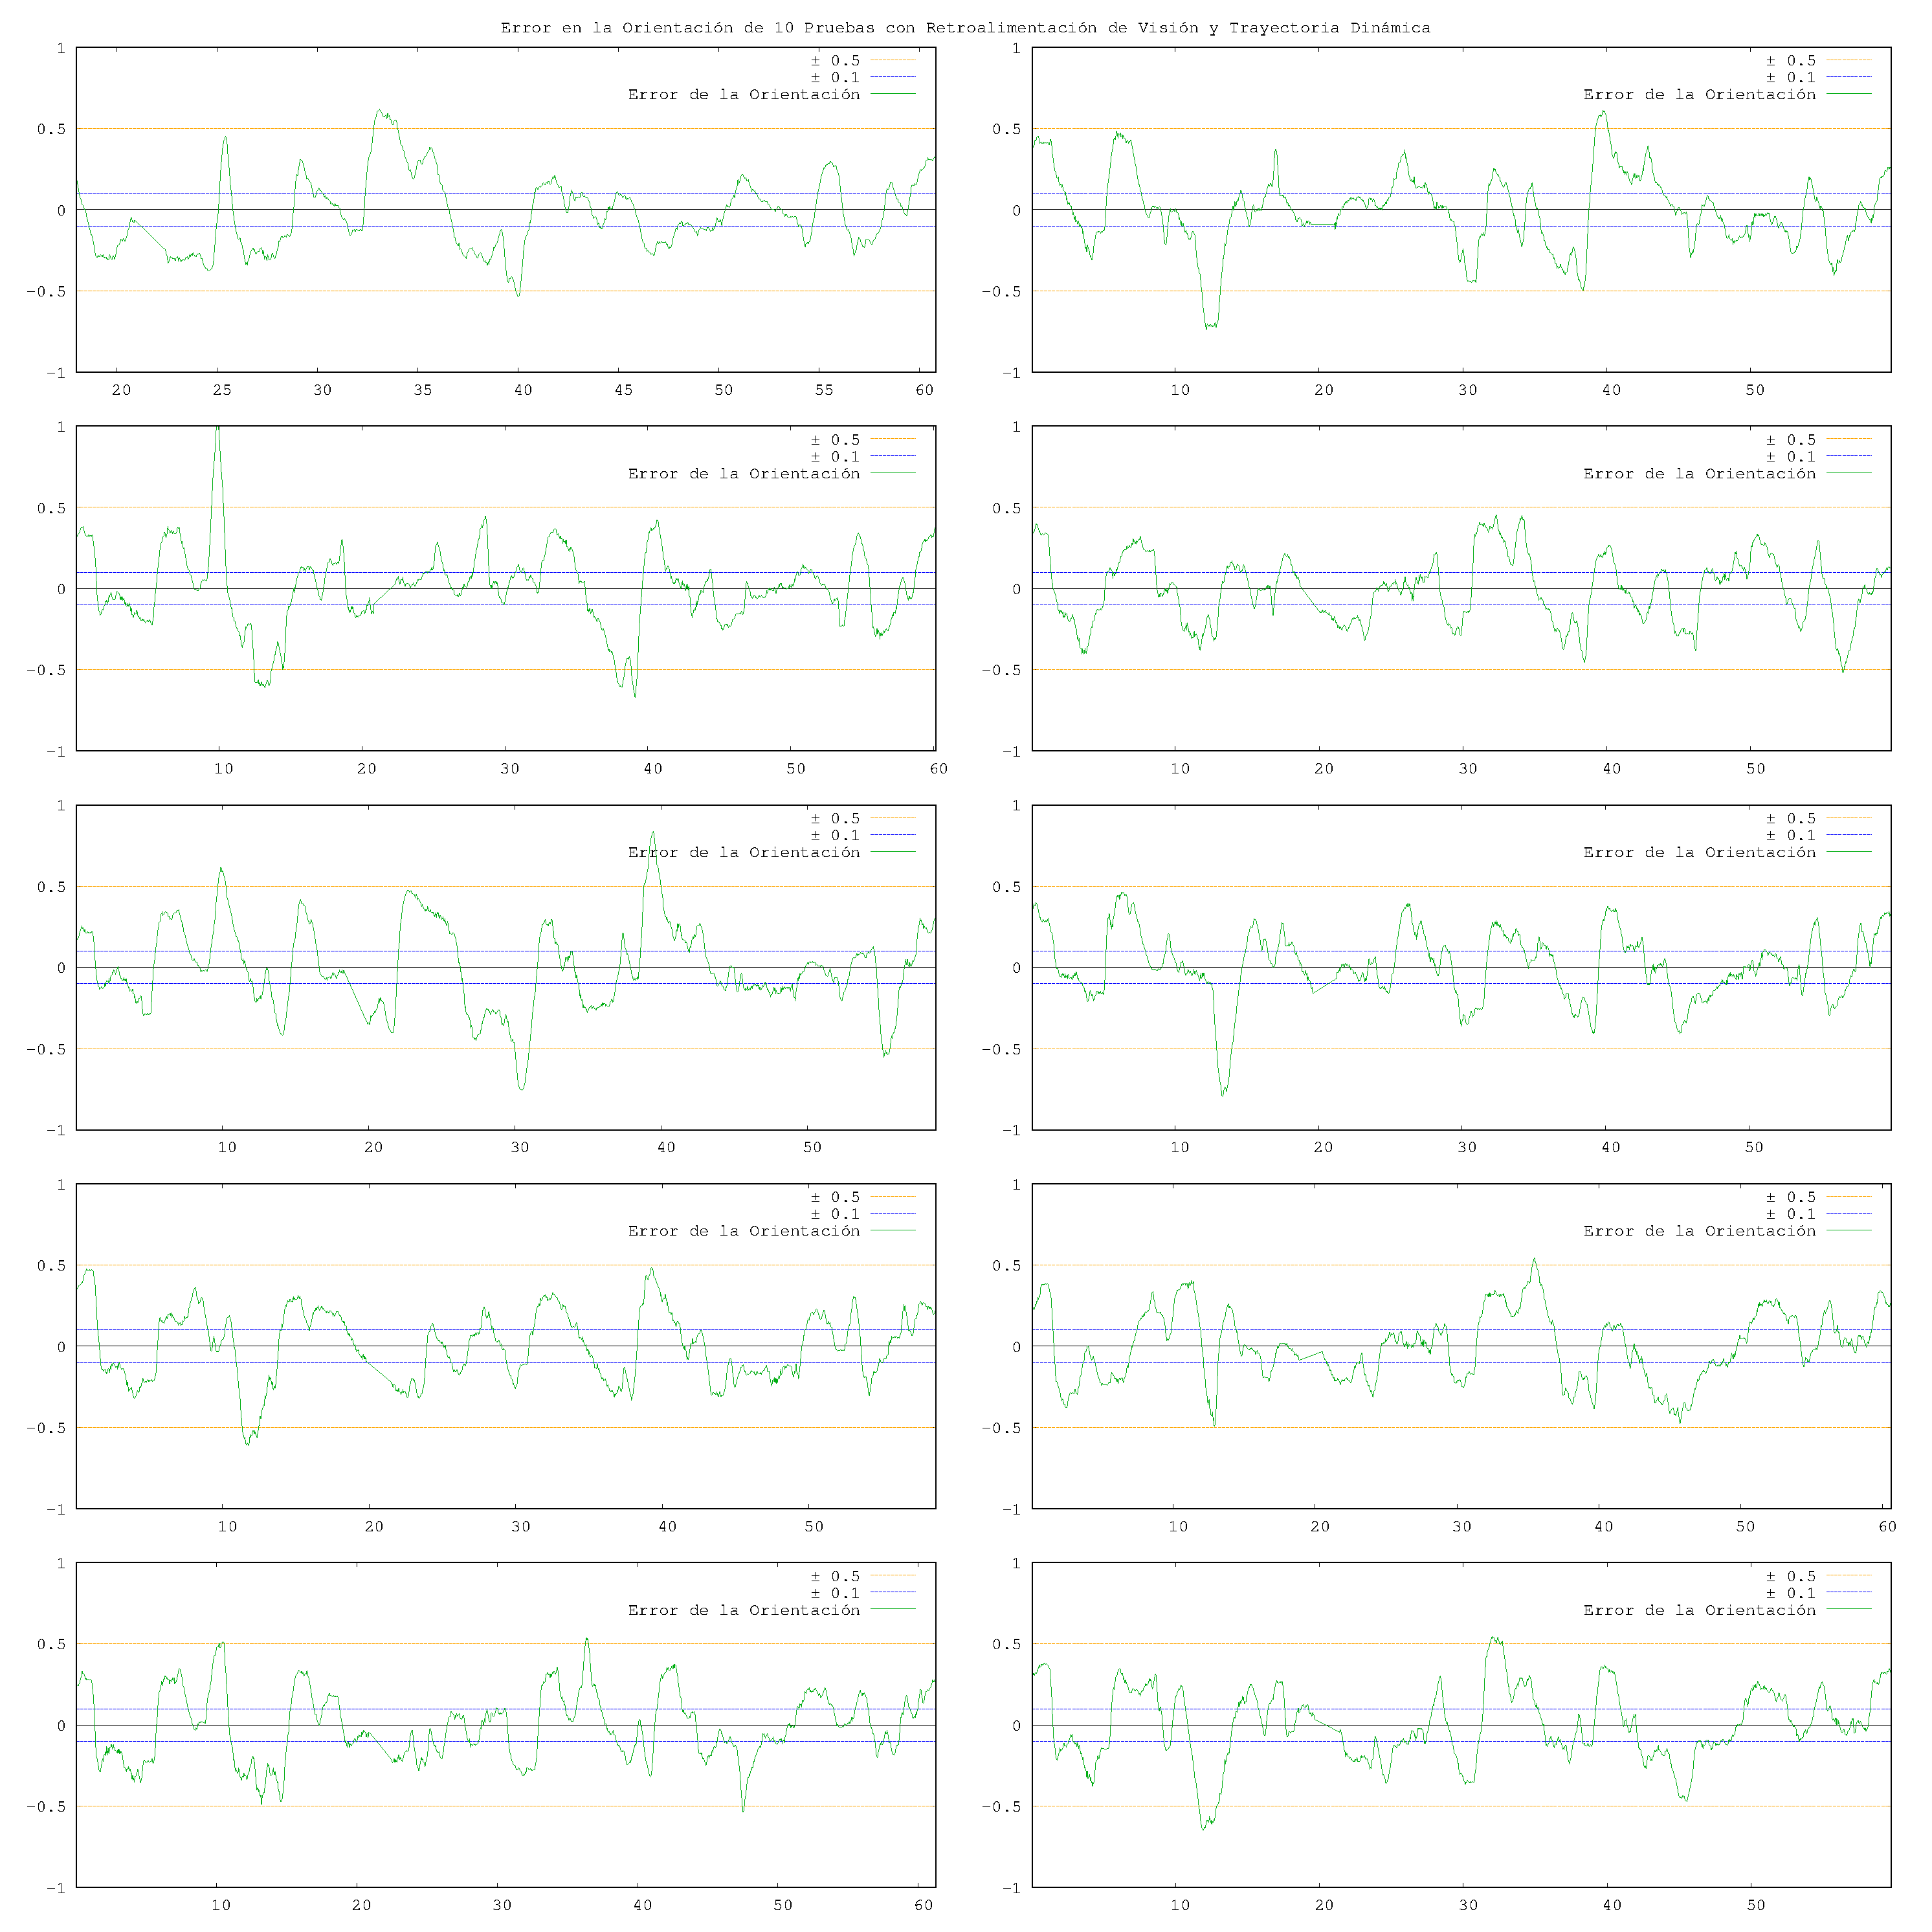
\includegraphics[height=3cm,width=8cm]{8pts260517-with_vision-multi-theta.eps}
%   \caption{Velocidades Deseadas vs Velocidades Reales}
%   \label{fig:orient_vision_multi}
% \end{figure}
%%%%%%%%%%%%%%%% end figure %%%%%%%%%%%%%%%%%%% 
%%%%%%%%%%%%%%%%%%%%%%%%%%%%%%%%%%%%%%%%%%%%%%%%%%%%%%%%%%%%%%%%%%%%%%
%%%%%%%%%%%%%%%%%%%%%%%%%%%%%%%%%%%%%%%%%%%%%%%%%%%%%%%%%%%%%%%%%%%%%%
%%%%%%%%%%%%%%% begin table   %%%%%%%%%%%%%%%%%%%%%%%%%%
% \begin{table}[t]
% \caption{THE TABLE CAPTION USES CAPITAL LETTERS, TOO.}
% \begin{center}
% \label{table_AMRob}
% \begin{tabular}{c l l}
% & & \\ % put some space after the caption
% \hline
% Example & Time & Cost \\
% \hline
% 1 & 12.5 & \$1,000 \\
% 2 & 24 & \$2,000 \\
% \hline
% \end{tabular}
% \end{center}
% \end{table}
%%%%%%%%%%%%%%%% end table %%%%%%%%%%%%%%%%%%% 




%%%%%%%%%%%%%%%%%%%%%%%%%%%%%%%%%%%%%%%%%%%%%%%%%%%%%%%%%%%%%%%%%%%%%%
% All tables should be numbered consecutively and  captioned; the caption should use all capital letters, and centered above the table as shown in Table~\ref{table_AMRob}. The body of the table should be no smaller than 7 pt.  There should be a minimum two line spaces between tables and text.
%%%%%%%%%%%%%%%%%%%%%%%%%%%%%%%%%%%%%%%%%%%%%%%%%%%%%%%%%%%%%%%%%%%%%%
\section*{CONCLUSIONES}
\label{sec:conclusiones}
Se presentó el diseño de un sistema robot omnidireccional para su uso en aplicaciones colaborativas. La arquitectura del sistema fue probada con un robot que cumple las especificaciones de \emph{Small Size League} de la RoboCup, El diseño modular del sistema permite intercambiar componentes para otras aplicaciones gracias a su integración con ROS.

Los experimentos realizados muestran que las distintas capas de control del robot tienen un desempeño adecuado. Esto nos permite utilizar los robots en la aplicación de pruebas y otras que requieran trabajo colaborativo. Para esto se requeriría desarrollar los módulos de ROS necesarios o incorporar otros.

Como trabajo futuro se propone un método de sintonización automático para el sistema de control. Adicionalmente, es necesario refinar los algoritmos implementados de planificación de tareas y de planificación de movimientos.

%\subsection*{Notes for the Practicioner} \TODO{Cambiar nombre por uno adecuado}
%\TODO{escribir}

% \section*{FOOTNOTES\protect\footnotemark}
% \footnotetext{Examine the input file, asme2e.tex, to see how a footnote is given in a head.}

% Footnotes are referenced with superscript numerals and are numbered consecutively from 1 to the end of the paper\footnote{Avoid footnotes if at all possible.}. Footnotes should appear at the bottom of the column in which they are referenced.


%%%%%%%%%%%%%%%%%%%%%%%%%%%%%%%%%%%%%%%%%%%%%%%%%%%%%%%%%%%%%%%%%%%%%%
% \section*{CITING REFERENCES}

%%%%%%%%%%%%%%%%%%%%%%%%%%%%%%%%%%%%%%%%%%%%%%%%%%%%%%%%%%%%%%%%%%%%%%
% The AMRob reference format is defined in the authors kit provided by the AMRob.  The format is:

% \begin{quotation}
% {\em Text Citation}. Within the text, references should be cited in  numerical order 
% according to their order of appearance.  The numbered reference citation should be 
% enclosed in brackets.
% \end{quotation}

% The references must appear in the paper in the order that they were cited.  In addition, 
% multiple citations (3 or more in the same brackets) must appear as a `` [1-3]''.

% The bibliography style required by the AMRob is unsorted with entries appearing in the 
% order in which the citations appear. If that were the only specification, the standard 
% {\sc Bib}\TeX\ unsrt bibliography style could be used. Unfortunately, the bibliography 
% style required by the ASME has additional requirements (last name followed by first 
% name, periodical volume in boldface, periodical number inside parentheses, etc.) that 
% are not part of the unsrt style. Therefore, to get ASME bibliography formatting, you 
% must use the \verb+amrob.bst+ bibliography style file with {\sc Bib}\TeX. This file is 
% not part of the standard BibTeX distribution so you'll need to place the file someplace 
% where LaTeX can find it (one possibility is in the same location as the file being typeset).


% Here's where you specify the bibliography style file.
% The full file name for the bibliography style file 
% used for an ASME paper is asmems4.bst.
\bibliographystyle{amrob}


%%%%%%%%%%%%%%%%%%%%%%%%%%%%%%%%%%%%%%%%%%%%%%%%%%%%%%%%%%%%%%%%%%%%%%

%%%%%%%%%%%%%%%%%%%%%%%%%%%%%%%%%%%%%%%%%%%%%%%%%%%%%%%%%%%%%%%%%%%%%%
% \begin{acknowledgment}
% Este trabajo fue patrocinado por la Asociación Mexicana de Cultura A.C.
% \end{acknowledgment}

%%%%%%%%%%%%%%%%%%%%%%%%%%%%%%%%%%%%%%%%%%%%%%%%%%%%%%%%%%%%%%%%%%%%%%
% The bibliography is stored in an external database file
% in the BibTeX format (file_name.bib).  The bibliography is
% created by the following command and it will appear in this
% position in the document. You may, of course, create your
% own bibliography by using thebibliography environment as in
%
% \begin{thebibliography}{12}
% % ...
% \bibitem{itemreference} D. E. Knudsen.
% {\em 1966 World Bnus Almanac.}
% {Permafrost Press, Novosibirsk.}
% % ...
% \end{thebibliography}

% Here's where you specify the bibliography database file.
% The full file name of the bibliography database for this
% article is asme2e.bib. The name for your database is up
% to you.
\bibliography{local}

%%%%%%%%%%%%%%%%%%%%%%%%%%%%%%%%%%%%%%%%%%%%%%%%%%%%%%%%%%%%%%%%%%%%%%
\appendix       %%% starting appendix
% \section*{Appendix A: Head of First Appendix}
% Avoid Appendices if possible.

%%%%%%%%%%%%%%%%%%%%%%%%%%%%%%%%%%%%%%%%%%%%%%%%%%%%%%%%%%%%%%%%%%%%%%
% \section*{Appendix B: Head of Second Appendix}
% \subsection*{Subsection head in appendix}
% The equation counter is not reset in an appendix and the numbers will
% follow one continual sequence from the beginning of the article to the very end as shown in the following example.
% \begin{equation}
% a = b + c.
% \end{equation}

\end{document}
